\documentclass[english,9pt,aspectraio=169]{beamer}
\usepackage{etex}
\usetheme{uzhneu-en-informal}
%\usepackage{uarial}
\usepackage[T1]{fontenc}
\usepackage[utf8]{inputenc}
\RequirePackage{graphicx,ae}
\usepackage{bm}
\usepackage{fancybox,amssymb,color}
\usepackage{pgfpages}
\usepackage{booktabs}
\usepackage{verbatim}
\usepackage{animate}
\usepackage{numprint}
\usepackage{dsfont}
\usepackage{tikz}
\usepackage{amsmath,natbib}
\usepackage{mathbbol}
\usepackage{babel}
\usepackage{SweaveSlides}
\usepackage{multicol}
\usepackage{xcolor}


\usetheme{uzhneu-en-informal}
\DeclareMathOperator{\po}{Poisson}
\DeclareMathOperator{\G}{Gamma}
\DeclareMathOperator{\Be}{Beta}
\DeclareMathOperator{\logit}{logit}
\def\n{\mathop{\mathcal N}}

\definecolor{Gray}{RGB}{139,137,137}
\definecolor{darkred}{rgb}{0.8,0,0}
\definecolor{Green}{rgb}{0,0.8,0.3}
\definecolor{lightgreen}{rgb}{0,0.7,0.3}
\definecolor{Blue}{rgb}{0,0,1}
\def\myalert{\textcolor{darkred}}
\def\myref{\textcolor{Gray}}
\setbeamercovered{invisible}

\renewcommand{\baselinestretch}{1.2}
\beamertemplateballitem
\DeclareMathOperator{\cn}{cn} % Copy number
\DeclareMathOperator{\ccn}{ccn} % common copy number
\DeclareMathOperator{\p}{p} % common copy number
\DeclareMathOperator{\E}{E} % common copy number
\DeclareMathOperator{\given}{|} % common copy number
\def\given{\,|\,}
\def\na{\tt{NA}}
\def\nin{\noindent}
\pdfpageattr{/Group <</S /Transparency /I true /CS /DeviceRGB>>}
\def\eps{\varepsilon}

\renewcommand{\P}{\operatorname{\mathsf{Pr}}} % Wahrscheinlichkeitsmaß
\def\eps{\varepsilon}
\def\logit{\text{logit}}
%\newcommand{\E}{\mathsf{E}} % Erwartungswert
\newcommand{\Var}{\text{Var}} % Varianz
\newcommand{\NBin}{\text{NBin}}
\newcommand{\Po}{\text{Po}}
\newcommand{\N}{\mathsf{N}}

\newcommand{\hl}{\textcolor{red}}

\newcommand{\ball}[1]{\begin{pgfpicture}{-1ex}{-0.65ex}{1ex}{1ex}
\usebeamercolor[fg]{item projected}

{\pgftransformscale{1.75}\pgftext{\normalsize\pgfuseshading{bigsphere}}}
{\pgftransformshift{\pgfpoint{0pt}{0.5pt}}
\pgftext{\usebeamerfont*{item projected}{#1}}}
\end{pgfpicture}}%
\usepackage{multicol}
\newcommand{\ballsmall}[1]{\begin{pgfpicture}{-1ex}{-0.65ex}{.2ex}{.2ex}

{\pgftransformscale{1}\pgftext{\normalsize\pgfuseshading{bigsphere}}}
{\pgftransformshift{\pgfpoint{0pt}{0.5pt}}
\pgftext{\usebeamerfont*{item projected}{#1}}}
\end{pgfpicture}}%



\begin{document}

\fboxsep5pt

\frame{
\title[]{ \centering \Huge Kurs Bio144: \\
Datenanalyse in der Biologie}%\\[.3cm]
\author[Stefanie Muff, Owen L.\ Petchey]{\centering Stefanie Muff  \& Owen L.\ Petchey }
%\institute[]{Institute of Social and Preventive Medicine \\ Institute of Evolutionary Biology and Environmental Studies}
\date[]{Week 5: ANOVA \\ 23./24. March 2017}


\maketitle
}


\frame{\frametitle{Overview (todo: check)}
\begin{itemize}
\item One-way ANOVA  
\item Post-hoc tests and contrasts
\item Two-way ANOVA 
\item ANOVA as special cases of a linear model \\[6mm]
\end{itemize}

Note: \\[2mm]
ANOVA = ANalysis Of VAriance  (Varianzanalyse)\\
}


\frame{\frametitle{Course material covered today}
\begin{itemize}
\item Chapter 12 from ``Statistische Datenenalyse -- Eine Einf\"uhrung f\"ur Naturwissenschaftler''
\item ``The new Statistics with R'' chapter 2 (ANOVA)
\end{itemize}
}

\frame[containsverbatim]{\frametitle{Recap of the linear regression model}
to do 
}


\frame{\frametitle{ANOVA and ANCOVA}
ANOVA = Varianzanalyse\\
ANCOVA = Kovarianzanalyse \\[2mm]

Introduction by Sir R.\ A.\ Fisher (1890-1962). He worked at the agricultural research station in Rothamstead (England). AN(C)OVA are/were therefore traditionally used to analyze agricultural experiments.\\[6mm]

Questions of AN(C)OVA:
\begin{itemize}
\item Generally: Are the means of twor or more groups different?\\[2mm]
\item Example: Are different plant breeds different in important aspects (e.g., yiels / Ertrag)?\\[2mm]
\item Example: What is the influence of different treatments on plants (Biology) or patients (Medicine)? \\[2mm]
\end{itemize}
}


\frame[containsverbatim]{\frametitle{Beispiel: Ertragspotential bei Hybrid-Mais mit erh\"ohter Pilzbrand-Resistenz}
\vspace{-4mm}
{\scriptsize (Source: W. Blanckenhorn, UZH)}\\[2mm]

Es wurden 4 Hybrid-Mais-Sorten angebaut und ihr K\"ornerertrag ermittelt. Jede Sorte wurde an 5 Orten angepflanzt.\\[2mm]

{\bf Frage:} Unterscheiden sich die Hybrid-Mais-Sorten im Ertrag? \\[2mm]
{\scriptsize \myalert{Achtung:} Die Frage bezieht sich auf \emph{irgendeinen} Unterschied. Pr\"aziser k\"onnte man fragen, ob sich irgendeine der Sorten von den anderen unterscheidet?}
\vspace{-5mm}
%
\begin{center}
\setkeys{Gin}{width=0.5\textwidth}
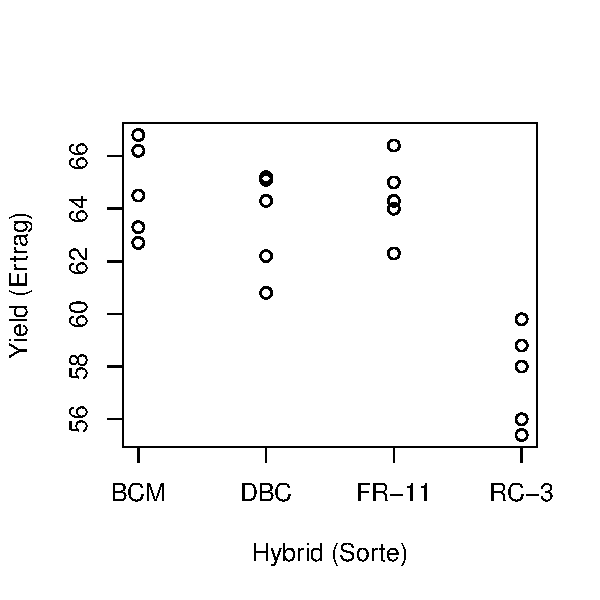
\includegraphics{Bio144_2017_week5-002}
\end{center}

ANOVA hilft uns, zu testen, ob es einen Unterschied zwischen den Sorten gibt.
}

\frame{\label{sl:naive}
{\bf Naive idea:} 
To carry out pairwise $t$-tests between any two groups. \\[4mm]

\begin{enumerate}
\item How many tests would this imply?\\[2mm]
\item Why is this not a very clever idea? \\[8mm]
\end{enumerate}

\pause
(Generally, the number of pairwise tests can be calculated by $g(g-1)/2$, where $g$=number of groups.)
}

% \frame{
% {\bf Better idea:} Formulate a model that is able to test whether there is an \myalert{overall difference between the groups.}
% 
% }


\frame[containsverbatim]{
{\bf Better idea} 

Formulate a model that is able to \myalert{test simultaneously} whether there is an \myalert{overall difference between the groups.} That is, ask only {\bf one question!}\\[2mm]

This leads us to the\\[4mm]

\colorbox{lightgray}{\begin{minipage}{10cm}
{\bf Idea of the ANOVA analysis:} \\
Compare the variability within groups ($MS_E$) to the variability between the group means ($MS_G$).
\end{minipage}}
\vspace{-10mm}
\begin{center}
\setkeys{Gin}{width=0.5\textwidth}
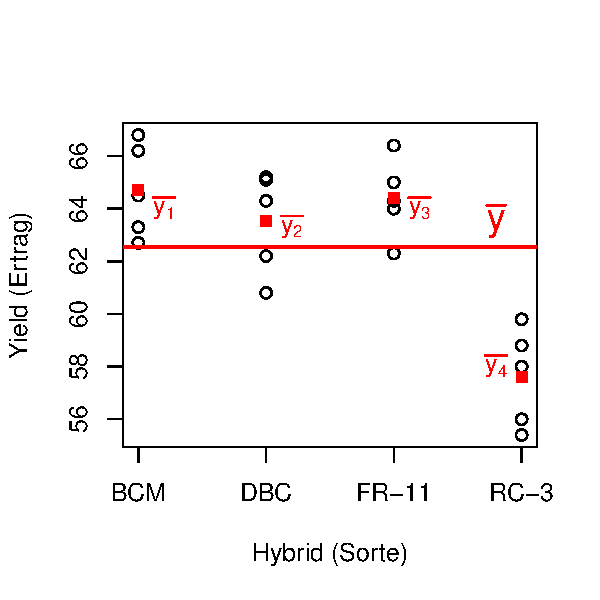
\includegraphics{Bio144_2017_week5-003}
\end{center}
}

\frame{
We formulate a model as follows:
\begin{eqnarray*}
y_{ij} = \mu_i + e_{ij} \ ,
\end{eqnarray*}
where 
\begin{itemize}
\item $y_{ij}$= ``Ertrag der $j$-ten Pflanze der Sorte $i$''
\item $\mu_i$=``Mittlerer Ertrag der Sorte $i$''
\item $e_{ij}\sim\N(0,\sigma_e^2)$ is an independent error term. \\[4mm]
\end{itemize}

Typically, this is rewritten as
\begin{eqnarray*}
y_{ij} = \mu + \beta_i + e_{ij} \ ,
\end{eqnarray*}
where $\mu + \beta_i = \mu_i$ from above, thus the {\bf group mean} of group $i$.
}

\frame{\frametitle{Single factor ANOVA (Einfaktorielle Varianzanalyse)}
\myalert{More generally}, this leads us to the \myalert{single factor ANOVA:}\\[2mm]

\colorbox{lightgray}{\begin{minipage}{10cm}
Assume we have $g$ groups and in each group $i$ there are $n_i$ measurements of some variable of interest, denoted as $y$. The model is then given as
\begin{eqnarray}
y_{ij} = \mu + \beta_i + e_{ij} \quad \text{for }\quad  i &=&1,\ldots ,g \ , \label{eq:aov}  \\
j &=& 1,\ldots, n_i , \nonumber\\ 
e_{ij} &\sim& \N(0,\sigma_e^2) \quad i.i.d. \nonumber
\end{eqnarray}
\end{minipage}}
~\\[2mm]

\begin{itemize}
\item $\mu$ plays the role of the \myalert{intercept} $\beta_0$ in standard regression models.
\item The estimation of $\mu$, $\beta_2$, \ldots, $\beta_g$ is again done by \myalert{least squares minimization}.
\item The $e_{ij} \sim \N(0,\sigma_e^2) \quad i.i.d.$ assumption is again crucial, so \myalert{model checking} will be needed again.
\end{itemize}

}


\frame{

Attention: Model \eqref{eq:aov} is overparameterized, thus an additional constraint is needed! Most popular:\\[2mm]

\begin{itemize}
\item $\beta_1=0$ (\myalert{treatment contrast}; default in R).
\item $\sum_i\beta_i = 0$ (\myalert{sum-to-zero contrast}).
\end{itemize}
}


\frame{\frametitle{The ANOVA test: The $F$-test}
Test now \emph{globally} if the groups differ. That is:\\

\begin{eqnarray*}
H_0 &:& \mu_1=\mu_2=\ldots = \mu_g  \quad \text{or, equivalently} \quad  \beta_1=\beta_2 = \ldots = \beta_g   \\[2mm]
H_1 &:& \text{At least two groups are different}
\end{eqnarray*}

~\\[2mm]
To test if more than one parameter in a regression model is =0 at the same time, we have used the {\bf $F$-test} in linear regression -- and we also need the $F$-test here!\\[2mm]

To derive the ingredients of the $F$-test, we again look at the decomposition of variance:
}

\frame{\frametitle{Variance decomposition}
(Remember this idea from week 3, slide 24, and replace $\hat{y_{ij}}$ by $\overline{y}_{\cdot i}$)

\begin{eqnarray*}
SS_{total} &=&  SS_{\text{between groups}} \qquad +\qquad SS_{\text{within groups}} \\
\sum_{i=1}^g \sum_{j=1}^{n_i} (y_{ij}-\overline{y})^2 & = &  \sum_{i=1}^g {n_i(\overline{y}_{\cdot i} - \overline{y})^2} \quad  + \quad
\sum_{i=1}^g \sum_{j=1}^{n_i}  (y_{ij} - \overline{y}_{\cdot i} )^2\\[4mm]
\text{Degrees of freedom:} \\
n-1 &= &   (g-1) \qquad  + \qquad (n-g)
\end{eqnarray*}
~\\


From this:
\colorbox{lightgray}{\begin{minipage}{10cm}
\begin{equation*}
\left.
\begin{array}{c}
MS_G = \frac{SS_{\text{between}}}{g-1} \\[2mm]
MS_E = \frac{SS_{\text{within}}}{n-g}
\end{array}
\right\}
\Rightarrow F = \frac{MS_G}{MS_E} \quad\text{is } \sim F_{g-1,n-g} \text{  distributed.} 
\end{equation*}
\end{minipage}}
}



\frame{\frametitle{Interpretation of the $F$ statistic}
\begin{itemize}
\item $MS_G$: Quantifies the variability {\bf between} groups.
\item $MS_E$: Quantifies the variability {\bf within} groups.\\[4mm]
\end{itemize}

Thus $F = \frac{MS_G}{MS_E}$ is large when $MS_G$ is ``large'' with respect to $MS_E$. The larger $F$, the more likely that $H_0$ is false. \\[4mm]

\begin{itemize}
\item $F$ increases 
\begin{itemize}
\item when the group means become more different, or
\item when the variability within groups decreases.
\end{itemize}
\item On the other hand, $F$decreases
\begin{itemize}
\item when the group means become more similar, or
\item when the variability within groups increases.
\end{itemize}
\end{itemize}

\href{http://onlinestatbook.com/stat_sim/one_way/index.html}
{\beamergotobutton{ANOVA App}}
}


\frame{\frametitle{The ANOVA table}
An overview of the results is typically given in an ANOVA table (Varianzanalyse-Tabelle):\\[6mm]

\begin{tabular}{llllll}
Variation & df & SS & MS = SS/df & F & $p$ \\ 
 \hline
 Between groups & $g-1$ & $SS_G$  &  $MS_G$ & $\frac{MS_G}{MS_E}$ & $\P(F_{g-1,n-g}>|F|))$\\
 Within groups &  $n-g$ & $SS_E$ & $MS_E$ & \\ 
 \hline 
 Total & $n-1$ & $SS_{\text{total}}$ & \\
 \hline 
\end{tabular}
}


\frame[containsverbatim]{\frametitle{Hybrid-Mais example -- Data}
The data look like this:\\[7mm]

\begin{tabular}{l@{\hspace{-7cm}}l}
\begin{Schunk}
\begin{Sinput}
> d.mais[,]
\end{Sinput}
\begin{Soutput}
   HYBRID LOCATION YIELD
1   FR-11       NW  62.3
2   FR-11       NE  64.0
3   FR-11        C  64.3
4   FR-11       SE  65.0
5   FR-11       SW  66.4
6     BCM       NW  63.3
7     BCM       NE  62.7
8     BCM        C  66.2
9     BCM       SE  66.8
10    BCM       SW  64.5
11    DBC       NW  60.8
12    DBC       NE  64.3
13    DBC        C  65.2
14    DBC       SE  62.2
15    DBC       SW  65.1
16   RC-3       NW  55.4
17   RC-3       NE  56.0
18   RC-3        C  59.8
19   RC-3       SE  58.0
20   RC-3       SW  58.8
\end{Soutput}
\end{Schunk}
&
\begin{Schunk}
\begin{Sinput}
> str(d.mais)
\end{Sinput}
\begin{Soutput}
'data.frame':	20 obs. of  3 variables:
 $ HYBRID  : Factor w/ 4 levels "BCM","DBC","FR-11",..: 3 3 3 3 3 1 1 1 1 1 ...
 $ LOCATION: Factor w/ 5 levels "C","NE","NW",..: 3 2 1 4 5 3 2 1 4 5 ...
 $ YIELD   : num  62.3 64 64.3 65 66.4 63.3 62.7 66.2 66.8 64.5 ...
\end{Soutput}
\end{Schunk}
\end{tabular}

}


\frame[containsverbatim]{\frametitle{Hybrid-Mais example -- Estimation}\label{sl:r.aov}
Using the \texttt{aov()} function in R directly estimates the ANOVA table:\\[4mm]

\begin{Schunk}
\begin{Sinput}
> r.mais <- aov(YIELD ~ HYBRID, d.mais)
> summary(r.mais)
\end{Sinput}
\begin{Soutput}
            Df Sum Sq Mean Sq F value   Pr(>F)    
HYBRID       3 167.44   55.81   17.68 2.47e-05 ***
Residuals   16  50.51    3.16                     
---
Signif. codes:  0 ‘***’ 0.001 ‘**’ 0.01 ‘*’ 0.05 ‘.’ 0.1 ‘ ’ 1
\end{Soutput}
\end{Schunk}
~\\[4mm]

Here: $F=17.68$ is $F$-distributed with 3 and 16 degrees of freedom, and the $p$-value of the test $\beta_1=\beta_2=\beta_3=\beta_4$ is $<0.0001$.\\[4mm]

\colorbox{lightgreen}{\begin{minipage}{10cm}
Conclusion: the four groups are clearly different!
\end{minipage}}

~\\[2mm]
{\bf Exercise:} Look at the table a bit closer. How are \texttt{Df}, \texttt{Sum Sq}, \texttt{Mean Sq}, \texttt{F value} and \texttt{Pr(<F)} related? 
}

\frame[containsverbatim]{
The $F$-distribution with 3 and 16 degrees of freedom, as well as the estimated value $F$=17.68:

\setkeys{Gin}{width=0.6\textwidth}
\includegraphics{Bio144_2017_week5-007}
}

\frame{\frametitle{ANOVA as a special case of a linear model}
\colorbox{lightgreen}{\begin{minipage}{10cm}
The clou is: Model \eqref{eq:aov} is identical to the regression model with a factor covariate, see slides 36/37 from week 3. 
\end{minipage}}
~\\[4mm]
{\bf Interpretation: The levels of the factor are now the different group memberships.} \\
Thus (assuming $\beta_1=0$):\\

\begin{equation*}
 y_{ij} = \left\{
\begin{array}{ll}
\mu + e_{ij}, & \text{for group } 1\\
\mu  + \beta_2  + e_{ij}, &  \text{for group } 2\\
...\\
\mu  + \beta_g + e_{ij}, &  \text{for group } g \ ,
\end{array}\right.
\end{equation*} 
~\\[4mm]
and $\hat{y}_{ij} = \overline{y}_{\cdot i} = \mu + \beta_i$ can be interpreted as the predicted value.\\[2mm]



}

\frame[containsverbatim]{
It is therefore possible to perform an ANOVA with the \texttt{lm()} function in R and obtain the same results, either by looking at the summary table:\\[4mm]

\begin{Schunk}
\begin{Sinput}
> r.lm <- lm(YIELD~HYBRID,d.mais)
> summary(r.lm)
\end{Sinput}
\begin{Soutput}
Call:
lm(formula = YIELD ~ HYBRID, data = d.mais)

Residuals:
   Min     1Q Median     3Q    Max 
 -2.72  -1.45   0.15   1.52   2.20 

Coefficients:
            Estimate Std. Error t value Pr(>|t|)    
(Intercept)  64.7000     0.7946  81.427  < 2e-16 ***
HYBRIDDBC    -1.1800     1.1237  -1.050    0.309    
HYBRIDFR-11  -0.3000     1.1237  -0.267    0.793    
HYBRIDRC-3   -7.1000     1.1237  -6.318 1.02e-05 ***
---
Signif. codes:  0 ‘***’ 0.001 ‘**’ 0.01 ‘*’ 0.05 ‘.’ 0.1 ‘ ’ 1

Residual standard error: 1.777 on 16 degrees of freedom
Multiple R-squared:  0.7683,	Adjusted R-squared:  0.7248 
F-statistic: 17.68 on 3 and 16 DF,  p-value: 2.474e-05
\end{Soutput}
\end{Schunk}
}

\frame[containsverbatim]{
...or by generating the ANOVA table for an lm object:\\[6mm]

\begin{Schunk}
\begin{Sinput}
> anova(r.lm)
\end{Sinput}
\begin{Soutput}
Analysis of Variance Table

Response: YIELD
          Df  Sum Sq Mean Sq F value    Pr(>F)    
HYBRID     3 167.441  55.814  17.681 2.474e-05 ***
Residuals 16  50.508   3.157                      
---
Signif. codes:  0 ‘***’ 0.001 ‘**’ 0.01 ‘*’ 0.05 ‘.’ 0.1 ‘ ’ 1
\end{Soutput}
\end{Schunk}

~\\[4mm]
Compare the output with the previous slide and slide \ref{sl:r.aov} for a while....
}

\frame[containsverbatim]{\frametitle{Testing modelling assumptions}
Tukey-Anscombe (TA) and QQ plots are useful again:
\setkeys{Gin}{width=0.9\textwidth}
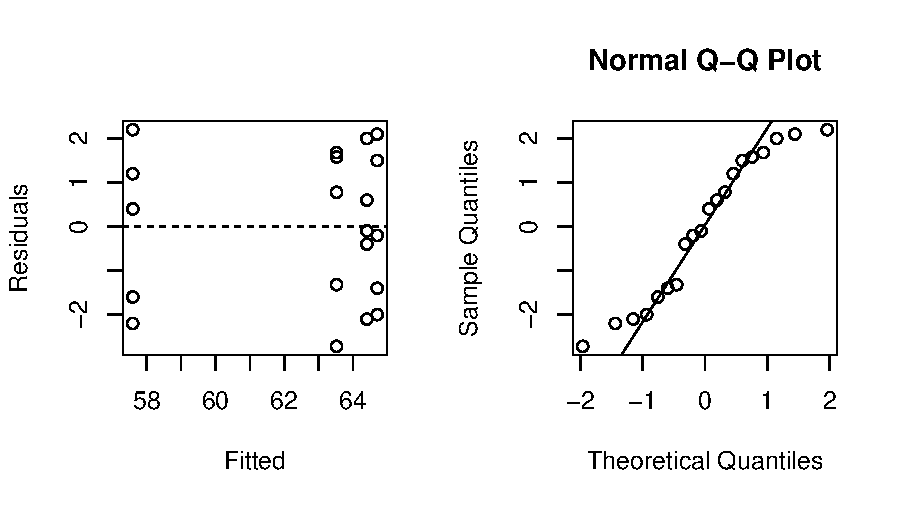
\includegraphics{Bio144_2017_week5-TA1}
}

\frame[containsverbatim]{\frametitle{Exercise: Ern\"ahrung und Blutzucker}
Remember example 3 from the first week: \\[2mm]
24 Personen werden in 4 Gruppen unterteilt. Jede Gruppe erh\"alt eine andere Di\"at \small{(DIAET)}. Es werden zu Beginn und am Ende (nach 2 Wochen) die Blutzuckerwerte gemessen. Die Differenz wird gespeichert \small{(BLUTZUCK)}.\\[2mm]
{\bf Frage:} Unterscheiden sich die Gruppen in der Ver\"anderung der Blutzuckerwerte?\\[3mm]

\begin{center}
\setkeys{Gin}{width=0.7\textwidth}
\begin{Schunk}
\begin{Sinput}
> par(mfrow=c(1,2))
> plot(BLUTZUCK ~ DIAET,d.blz,xaxt="n",main="Streudiagramm")
> axis(1,1:4)
> boxplot(BLUTZUCK ~ DIAET,d.blz,xaxt="n",xlab="DIAET",main="Boxplot")
> axis(1,1:4)
\end{Sinput}
\end{Schunk}
\includegraphics{Bio144_2017_week5-blz_plot}
\end{center}
}

\frame[containsverbatim]{
Interpret the results and the residual plots:\\[4mm]
\begin{Schunk}
\begin{Sinput}
> d.blz$DIAET <- as.factor(d.blz$DIAET)
> summary(aov(BLUTZUCK ~ DIAET,d.blz))
\end{Sinput}
\begin{Soutput}
            Df Sum Sq Mean Sq F value  Pr(>F)   
DIAET        3  31.56   10.52   7.514 0.00148 **
Residuals   20  28.00    1.40                   
---
Signif. codes:  0 ‘***’ 0.001 ‘**’ 0.01 ‘*’ 0.05 ‘.’ 0.1 ‘ ’ 1
\end{Soutput}
\end{Schunk}

\begin{center}
\setkeys{Gin}{width=0.77\textwidth}
\includegraphics{Bio144_2017_week5-blz_plot_res}
\end{center}
}

\frame{\frametitle{Multiple comparisons, multiple tests}
To remember:
\begin{itemize}
\item The $F$-Test is used to check whether \myalert{any two group means} differ. 
\item Using pairwise tests is not a very good idea (see slide \ref{sl:naive}), because this leads to a \myalert{multiple testing problem}: \\[2mm]

 \colorbox{lightgreen}{\begin{minipage}{10cm}
When many tests are carried out, the probability to find a ``significant'' result {\bf by chance} increases.
\end{minipage}}
~\\[6mm]
For instance, for four groups there are $4\cdot 3/2= 6$ pairwise combinations that could be tested. The probability to find \emph{at least one result by chance} is much higher than the 5\% error level!!!\\[6mm]
\end{itemize}

}


\frame{\frametitle{Post-hoc tests}
{\bf Still:} If the test $\beta_1=\beta_2=\ldots= \beta_g=0$ is rejected, one is often interested 
\begin{enumerate}
\item in finding the actual group(s) that deviate(s) from the others.
\item in estimates of the pairwise differences.\\[6mm]
\end{enumerate}

Several methods to circumvent the problem of  too many ``significant'' test results (type-I error) have been proposed. The most prominent ones are:\\[2mm]
\colorbox{lightgray}{\begin{minipage}{10cm}
\begin{itemize}
\item Bonferroni correction
\item Tukey {\bf h}onest {\bf s}ignificant {\bf d}ifferences (HSD) approach
\item Fisher {\bf l}east {\bf s}ignificant {\bf d}ifferences (LSD) approach
\end{itemize}
\end{minipage}}
}

\frame{\frametitle{}
\myalert{\bf Bonferroni correction}\\[2mm]

{\bf Idea:} If a total of $m$ tests are carried out, simply divide the type-I error level $\alpha_0$ (often 5\%) such that

$$\alpha = \alpha_0 / m \ .$$


\myalert{\bf Tukey HSD approach}\\[2mm]

{\bf Idea:} Take into account the distribution of \emph{ranges} (max-min) and design a new test. \\[6mm]

\myalert{\bf Fisher's LSD approach}\\[2mm]

{\bf Idea:} Adjust the idea of a two-sample test, but use a larger variance (namely the pooled variance of all groups).
}

\frame[containsverbatim]{
Calculate the pairwise differences and tests with adjustments for the ``Blutzucker'' example:

\begin{multicols}{2}
Differences:\\
\begin{tabular}{l|ccc}
& 1 & 2 & 3\\
\hline
2 & 1.2 &  & \\
3 & -1.1 & -2.3\\
4 & 1.9 & 0.7 & 3.0\\
\end{tabular}

~\\[4mm]
Bonferroni $p$-values: \\
\begin{tabular}{l|ccc}
& 1 & 2 & 3\\
\hline
2 & 0.57 &  & \\
3 & 0.74  &  0.02  \\
4 & 0.07   &1.00   & 0.002 \\
\end{tabular}

Tukey HSD $p$-values:\\
\begin{tabular}{l|ccc}
& 1 & 2 & 3\\
\hline
2 & 0.32 &  & \\
3 & 0.40 & 0.01\\
4 & 0.05 & 0.74 & 
0.001\\ 
\end{tabular}

~\\[4mm]
Fisher $p$-values: \\
\begin{tabular}{l|ccc}
& 1 & 2 & 3\\
\hline
2 & 0.09 &  & \\
3 & 0.12  &  0.003  \\
4 & 0.01   &0.32   & 3e-04 \\
\end{tabular}
\end{multicols}

\begin{itemize}
\item Bonferroni $p$-values are the most conservative (largest $p$).
\item Fisher $p$-values are the least conservative (smallest $p$).
\end{itemize}
}

\frame{\frametitle{Other contrasts}
Sometimes additional comparisons are of interest. For example, a new diet is to be compared to other, existing diets. \\[4mm]

In the ``Blutzucker'' example, this could be, for intance: ``Is diet 1 different from diets 2-4?'' \\[4mm]
}

\frame[containsverbatim]{\frametitle{Two-way ANOVA (Zweiweg-Varianzanalyse)}
Example {\scriptsize(from Hand et al. 1994 / Hothorn/Everitt ``A Handbook of Statistical Analyses Using R'')}: Experiment to study the weight gain of rats, depending on four diets. Protein amounts were either high or low, and the protein source was either beef or cereal. 10 rats for each diet were selected.\\[6mm]

{\bf Question:} How does diet affect weightgain? \\[6mm]

{\bf Complication:} This is a factorial design (gekreuzte Faktoren), because each combination of  protein source (beef/cereal) $\times$ level (high/low) is present (2$\times$2 groups).

Design: 
\begin{center}
\begin{tabular}{l|c|c|}
&beef & cereal \\
\hline
high & group 1 & group 2\\
\hline
low & group 3 & group 4\\
\hline
\end{tabular}
\end{center}
}

\frame[containsverbatim]{\label{sl:mean}
~\\
Start by looking at means and standard deviations in the groups, as well at a graphical description of the means: \\[2mm]
\begin{Schunk}
\begin{Sinput}
> tapply(weightgain$weightgain,list(weightgain$source,weightgain$type),FUN=mean)
\end{Sinput}
\begin{Soutput}
        High  Low
Beef   100.0 79.2
Cereal  85.9 83.9
\end{Soutput}
\begin{Sinput}
> tapply(weightgain$weightgain,list(weightgain$source,weightgain$type),FUN=sd)
\end{Sinput}
\begin{Soutput}
           High      Low
Beef   15.13642 13.88684
Cereal 15.02184 15.70881
\end{Soutput}
\end{Schunk}
~\\[2mm]
\begin{multicols}{2}
\setkeys{Gin}{width=0.5\textwidth}
\begin{Schunk}
\begin{Sinput}
> plot.design(weightgain)
\end{Sinput}
\end{Schunk}
\includegraphics{Bio144_2017_week5-018}
\begin{itemize}
\item Protein source (beef/cereal) seems less important than the amount (high/low).
\item Variances seem to be equal in the four groups.
\end{itemize}
\end{multicols}
}


\frame{\frametitle{Two-way ANOVA -- The model}

In the presence of a \myalert{factorial design}, the idea is to add separate effects $\beta_i$ (here $i=1,2$) and $\gamma_j$ (here $j=1,2$) for the $i$th level of the first factor and the $j$th level of the second factor:\\[5mm]

\colorbox{lightgray}{\begin{minipage}{10cm}
Assume we have a factorial design with two factors $\beta_i$ and $\gamma_j$, then the $k$th outcome in the group of $i$ and $j$, $y_{ijk}$ is modelled as
\begin{eqnarray}
y_{ijk} = \mu + \beta_i + \gamma_j +  e_{ijk} \quad \text{with} \quad e_{ijk} &\sim& \N(0,\sigma_e^2) \quad i.i.d. \nonumber
\end{eqnarray}
\end{minipage}}
~\\[5mm]
{\scriptsize
Again, additionl constraints are needed!
\begin{itemize}
\item $\beta_1=\gamma_1=0$ (\myalert{treatment contrast}; default in R).
\item $\sum_i\beta_i = \sum_i\gamma_i = 0$ (\myalert{sum-to-zero contrast}).
\end{itemize}
}
}



\frame[containsverbatim]{\frametitle{Two-way ANOVA in R}
In R, a two-way ANOVA is as simple as one-way ANOVA, just add another variable:\\[4mm]
\begin{Schunk}
\begin{Sinput}
> r.aov <- aov(weightgain ~ source + type,weightgain)
> summary(r.aov)
\end{Sinput}
\begin{Soutput}
            Df Sum Sq Mean Sq F value Pr(>F)  
source       1    221   220.9   0.915  0.345  
type         1   1300  1299.6   5.383  0.026 *
Residuals   37   8933   241.4                 
---
Signif. codes:  0 ‘***’ 0.001 ‘**’ 0.01 ‘*’ 0.05 ‘.’ 0.1 ‘ ’ 1
\end{Soutput}
\end{Schunk}
~\\[4mm]

Interpretation: There seems to be a difference between low and high amounts of protein. \\[6mm]

However: what if the additive model does not hold?
}


\frame[containsverbatim]{
A so-called \myalert{interaction plot} (\texttt{interaction.plot()} in R) helps to understand if the additive model is reasonable:\\[2mm]

\setkeys{Gin}{width=0.6\textwidth}
\includegraphics{Bio144_2017_week5-020}

The lines are \myalert{not parallel}, indicating that \myalert{there is an interaction} between type and source!\\
{\scriptsize Note: if the additive model $\beta_i + \gamma_j$ holds, the lines would be parallel.}
}


\frame{\frametitle{Two-way ANOVA with interaction}
\begin{itemize}
\item If the purely additive model is not correct, a more general model with an interaction term $(\beta\gamma)_{ij}$ may be used:\\[2mm]

\colorbox{lightgray}{\begin{minipage}{10cm}
\begin{eqnarray}
y_{ijk} = \mu + \beta_i + \gamma_j + (\beta\gamma)_{ij} + e_{ijk} \quad \text{with} \quad e_{ijk} &\sim& \N(0,\sigma_e^2) \quad i.i.d. \nonumber
\end{eqnarray}
\end{minipage}}
~\\[4mm]

\item As in linear regression, interactions allow for an \myalert{ interplay between the variables}. 
\item In the rats experiment, increasing the amount from low to high has a different effect in the beef than in the cereal diet.
\item Moreover: The plot on the previous slide shows that for the low amount of proteins case, the cereal diet leads to a larger average weight gain!
\end{itemize}
}


\frame[containsverbatim]{\frametitle{Two-way ANOVA in R -- Including an interaction}

Again the rats example, this time including the interaction term:\\[4mm]

\begin{Schunk}
\begin{Sinput}
> r.aov <- aov(weightgain ~ source * type,weightgain)
> summary(r.aov)
\end{Sinput}
\begin{Soutput}
            Df Sum Sq Mean Sq F value Pr(>F)  
source       1    221   220.9   0.988 0.3269  
type         1   1300  1299.6   5.812 0.0211 *
source:type  1    884   883.6   3.952 0.0545 .
Residuals   36   8049   223.6                 
---
Signif. codes:  0 ‘***’ 0.001 ‘**’ 0.01 ‘*’ 0.05 ‘.’ 0.1 ‘ ’ 1
\end{Soutput}
\end{Schunk}
~\\[4mm]

The coefficient estimates can be obtained as follows:\\[4mm]
\begin{Schunk}
\begin{Sinput}
> r.lm <- lm(weightgain ~ source * type,weightgain)
> summary(r.lm)$coef
\end{Sinput}
\begin{Soutput}
                     Estimate Std. Error   t value     Pr(>|t|)
(Intercept)             100.0   4.728577 21.148009 6.842420e-22
sourceCereal            -14.1   6.687218 -2.108500 4.201233e-02
typeLow                 -20.8   6.687218 -3.110411 3.644273e-03
sourceCereal:typeLow     18.8   9.457155  1.987913 5.446757e-02
\end{Soutput}
\end{Schunk}
}

\frame{
{\bf Interpretation of the coefficients} 
\myalert{This works in the same way as for categorical covariates in regression!} To see this, let us estimate the means from the model. From the above output, we have {\scriptsize [because of using treatment contrasts]}:\\[4mm]

$\hat\beta_{beef}=0$, $\hat\beta_{cereal}=-14.1$, \\
$\hat\gamma_{high}=0$, $\hat\gamma_{low}=-20.8$,\\
$\hat{(\beta\gamma)}_{cereal/low}=18.8$, $\hat{(\beta\gamma)}_{beef/high}=\hat{(\beta\gamma)}_{beef/low}=\hat(\beta\gamma)_{cereal/high}=0$.\\[4mm]

Therefore:\\[2mm]

\begin{tabular}{l l}
Group 1: beef / high &  $\hat{y}_{beef,high} = 100 + 0 + 0 + 0 = 100$\\
Group 2: cereal / high & $\hat{y}_{cereal,high} = 100 + (-14.1) + 0 + 0 = 85.9$\\
Group 3: beef / low &  $\hat{y}_{beef,low} = 100 + 0 + (-20.8) + 0 = 79.2$\\
Group 4: cereal / low & $\hat{y}_{cereal,low} = 100 + (-14.1) + (-20.8) + 18.8 = 83.9$\\[6mm]
\end{tabular}

Compare these values to slide \ref{sl:mean}!
}

\frame{
And finally, again, checking some modelling assumptions:
\begin{center}
\setkeys{Gin}{width=0.9\textwidth}
\includegraphics{Bio144_2017_week5-TA2}
\end{center}
}


\frame[containsverbatim]{\frametitle{Exercise: }
In an experiment the influence of four levels of fertilizer (DUENGER) on the yield (ERTRAG) on 5 species (SORTE) of crops was investigated. The data contains the following colums:\\
DUENGER (4 levels) \hspace{1cm} SORTE (5 levels) \hspace{1cm} ERTRAG \\[6mm]


\begin{multicols}{2}
The first 10 rows of the data:\\[2mm]
\begin{Schunk}
\begin{Sinput}
> d.duenger[1:10,]
\end{Sinput}
\begin{Soutput}
   DUENGER SORTE ERTRAG
1        1     1     14
2        1     1     15
3        1     1     15
4        2     1     20
5        2     1     25
6        2     1     23
7        3     1     35
8        3     1     31
9        3     1     32
10       4     1     52
\end{Soutput}
\end{Schunk}
~\\[6mm]

And the interaction plot:
\setkeys{Gin}{width=0.4\textwidth}
\includegraphics{Bio144_2017_week5-026}
\end{multicols}
}

\frame[containsverbatim]{
The interaction plot indicates that an interaction between SORTE and DUENGER is needed in the analysis. The results and residal plots are given as follows:\\[2mm]

\begin{Schunk}
\begin{Sinput}
> d.duenger$SORTE <- as.factor(d.duenger$SORTE)
> d.duenger$DUENGER <- as.factor(d.duenger$DUENGER)
> r.duenger <- aov(ERTRAG ~ DUENGER*SORTE,d.duenger)
> summary(r.duenger)
\end{Sinput}
\begin{Soutput}
              Df Sum Sq Mean Sq F value Pr(>F)    
DUENGER        3  35801   11934  580.71 <2e-16 ***
SORTE          4  27805    6951  338.26 <2e-16 ***
DUENGER:SORTE 12   7674     640   31.12 <2e-16 ***
Residuals     40    822      21                   
---
Signif. codes:  0 ‘***’ 0.001 ‘**’ 0.01 ‘*’ 0.05 ‘.’ 0.1 ‘ ’ 1
\end{Soutput}
\end{Schunk}

\setkeys{Gin}{width=0.7\textwidth}
\includegraphics{Bio144_2017_week5-028}
~\\
Interpretation? What is here the problem (look at the TA plot)? Ideas?
}

\frame[containsverbatim]{
Todo: don't show this slide previously!\\
Log-transform the response (ERTRAG) and repeat the analysis:\\[2mm]

\begin{Schunk}
\begin{Sinput}
> r.duenger2 <- aov(log(ERTRAG) ~ DUENGER*SORTE,d.duenger)
> summary(r.duenger2)
\end{Sinput}
\begin{Soutput}
              Df Sum Sq Mean Sq F value Pr(>F)    
DUENGER        3 11.692   3.897 854.050 <2e-16 ***
SORTE          4  8.520   2.130 466.785 <2e-16 ***
DUENGER:SORTE 12  0.093   0.008   1.696  0.105    
Residuals     40  0.183   0.005                   
---
Signif. codes:  0 ‘***’ 0.001 ‘**’ 0.01 ‘*’ 0.05 ‘.’ 0.1 ‘ ’ 1
\end{Soutput}
\end{Schunk}

\setkeys{Gin}{width=1\textwidth}
\includegraphics{Bio144_2017_week5-030}
}


\frame{\frametitle{Some remarks }
\begin{itemize}
\item The $t$-test to compare the mean of \myalert{two gropus} is a \myalert{special case of ANOVA}.\\[2mm]
\item ANOVA is a \myalert{special cases of the linear regression model}.\\[2mm]
\item ANOVA is often taught in separate lectures, although it could be integrated in a lecture on linear regression. \\[2mm]
\item ANOVA is traditionally most used to analyze \myalert{experimental data}.\\[2mm]
\end{itemize}
}



\frame{\frametitle{Summary}

}
% \frame{References:
% \bibliographystyle{Chicago}
% \bibliography{refs}
% }



\end{document}
